\newcommand{\denote}[1]{\lbrack\!\lbrack#1\rbrack\!\rbrack}
\newcommand{\emeaning}[1]{{\cal D}\lbrack\!\lbrack#1\rbrack\!\rbrack}

\lstset{ %
language=ML, % choose the language of the code
basicstyle=\footnotesize\ttfamily,       % the size of the fonts that are used for the code
keywordstyle=\color{Bittersweet},
%numbers=left,                   % where to put the line-numbers
%numberstyle=\tiny,      % the size of the fonts that are used for the line-numbers
%stepnumber=1,                   % the step between two line-numbers. If it is 1 each line will be numbered
%numbersep=5pt,                  % how far the line-numbers are from the code
%backgroundcolor=\color{white},  % choose the background color. You must add \usepackage{color}
showspaces=false,               % show spaces adding particular underscores
showstringspaces=false,         % underline spaces within strings
showtabs=false,                 % show tabs within strings adding particular underscores
frame=single,                   % adds a frame around the code
tabsize=2,                      % sets default tabsize to 2 spaces
captionpos=b,                   % sets the caption-position to bottom
breaklines=true,                % sets automatic line breaking
breakatwhitespace=false,        % sets if automatic breaks should only happen at whitespace
commentstyle=\itshape\color{MidnightBlue},
%escapeinside={\%*}{*)},         % if you want to add a comment within your code
}

%Formatting Commands
%-------------------
\newcommand{\R}[1]{\textrm{#1}}
\renewcommand{\k}[1]{\mathtt{#1}} % Code font in math mode.
%\newcommand{\code}[1]{\,{\tt #1}\,}
\newcommand{\tab}{\hspace*{1.5em}}
\newcommand{\conj}{~\wedge~}
\newcommand{\disj}{~\vee~}
\newcommand{\fixme}[1]{\fbox{\textsl{\bf #1}}}
\newcommand{\pairedup}{{\cal P}}
\newcommand{\sender}{{\cal S}}
\newcommand{\intrastate}{{\sf State}_{\sf intra}}
\newcommand{\intralabel}{{\sf Label}_{\sf intra}}
\newcommand{\SCFN}[1]{{\sc\footnotesize {#1}}}
\newcommand{\ready}{\R{\SCFN{Ready}}}
\newcommand{\done}{\R{\SCFN{Done}}}
\newcommand{\obs}{{\sf obs}}
\newcommand{\obsE}{{\sf ObsE}}
\newcommand{\restrict}[2]{[#1]_{#2}}
\newcommand{\filter}[2]{#1{\downarrow}_{#2}}
\newcommand{\isucc}[1]{~{\sf isucc}_{#1}~}
\newcommand{\synthesize}{\triangleright}
\newcommand{\One}{{\sf One}}
\newcommand{\All}{{\sf All}}
\newcommand{\rel}{\R{\SCFN{Rel}}}
\newcommand{\intraTraceSet}{\sf InTr^{\program}}
\newcommand{\cml}{\R{\SCFN{Cml}}}

%Attributes
%----------
\newcommand{\synchrony}{\sigma}
\newcommand{\fifo}{\phi}
\newcommand{\reliability}{\rho}
\newcommand{\ptop}{\pi}

%Classes
%-------
\newcommand{\SelectClass}{\mathbb{S}}
\newcommand{\ChannelClass}{\mathbb{C}}
\newcommand{\ChannelStateClass}{\mathbb{S}}
\newcommand{\ValueClass}{\mathbb{V}}
\newcommand{\NumberClass}{\mathbb{N}}
\newcommand{\ThreadClass}{\mathbb{T}}
\newcommand{\AttributeClass}{\mathbb{K}}
\newcommand{\ActionClass}[1]{\mathbb{A}_{#1}}

%Relations
%---------
\newcommand{\po}{\rightarrow_{po}} %Program order
\newcommand{\co}{\rightarrow_{co}} %Communication order
\newcommand{\mo}{\rightarrow_{mo}} %Match order
\newcommand{\bico}{\leftrightarrow_{co}} %Communication order
\newcommand{\cd}{\rightarrow_{cd}} %Channel dependence
\newcommand{\sw}{\rightarrow_{sw}} %Synchronizes-with
\newcommand{\td}{\rightarrow_{td}} %Thread dependence
\newcommand{\tr}{\rightarrow_{tr}} %Trace
\newcommand{\hb}{\rightarrow_{hb}} %Happens-before relation
\newcommand{\nhb}{\nrightarrow_{hb}} %Happens-before neg
\newcommand{\nbihb}{\nleftrightarrow_{hb}} %Bi-happens-before neg
\makeatletter
\def\twoheadrightarrowfill@{\arrowfill@\relbar\relbar\twoheadrightarrow}
\newcommand{\intratrans}[2][] {\ext@arrow035{13}\twoheadrightarrowfill@{#1}{#2}}
\newcommand{\intertrans}[1]{\xrightarrow{#1}}
\makeatother

%Execution
%---------
%\newcommand{\CommMatch}{{\sf M}}
\newcommand{\ActionSet}{{\sf A}}
\newcommand{\ChannelStates}{{\sf C}}
\newcommand{\program}{{\sf P}}
\newcommand{\Exec}{\langle \program, \allowbreak \ActionSet, \allowbreak \po, \allowbreak \co \rangle}
\newcommand{\E}{{\sf E}}

%% op semantics

\newcommand{\DepGraph}{\Gamma}
\newcommand{\ActionSoup}{\Delta}
\newcommand{\CommitSet}{\Omega}


\newcommand{\HLREL}[1]{\R{\textsf{HL-REL}}(#1)}
\newcommand{\LLREL}[1]{\R{\textsf{LL-REL}}(#1)}
\newcommand{\CML}[1]{\R{\textsf{CML}}(#1)}
\newcommand{\EP}{{\sf E'}}
\newcommand{\toto}{\rightarrow_{to}} 								%Total order
\newcommand{\totoP}{\rightarrow_{to'}} 							%Total order prime
\newcommand{\totoPP}{\rightarrow_{to''}} 						%Total order double prime
\newcommand{\so}{\rightarrow_{so}} 									%Spawn Order
\newcommand{\ko}{\rightarrow_{ko}} 									%C(K)ommit order

\newcommand{\rulelabel}[1]{\textrm{\sc {[#1]}}}
\newcommand{\RULE}[2]{\frac{\begin{array}{c}#1\end{array}}
                           {\begin{array}{c}#2\end{array}}}
\newcommand{\RULEONE}[1]{{\begin{array}{c}#1\end{array}}}

\newcommand{\OExec}[3]{\langle #1, #2 \rangle_{#3}}
\newcommand{\ExecP}{\langle {\sf P}, \ActionSet,\po,\co \rangle}
\newcommand{\PrgState}[2]{\langle (t,E[#1]) \;\|\; \threadsoup,#2 \rangle}

\newcommand{\trace}{\mathit{tr}}
\newcommand{\commit}[2]{\epsilon_{(#1,#2)}}

\newcommand{\wf}[1]{{\sf WF}(#1)}
\newcommand{\transOpAx}[2]{\opax(#1,#2)}

\newcommand{\filtera}[2]{#1{\downarrow}_{#2}}

\newcommand{\thread}{\mathit{T}}
\newcommand{\threadid}{\textsf{t}}
\newcommand{\spawn}{\textsf{spawn}}
\newcommand{\unit}{\textsf{unit}}
\newcommand{\threadsoup}{\overline{\mathit{T}}}
\newcommand{\threadsoupp}{\overline{\mathit{T'}}}
\newcommand{\eval}[1]{\mathit{E}[#1]}
\newcommand{\evaln}{\mathit{E}}
\newcommand{\chan}{\textsf{ch}}
\newcommand{\send}{\textsf{send}}
\newcommand{\recv}{\textsf{recv}}
\newcommand{\join}{\textsf{join}}
\newcommand{\con}{\textsf{Con}}
\newcommand{\prev}{\textsf{Prev}}
\newcommand{\fresh}{\textsf{fresh}}
\newcommand{\print}{\textsf{print}}
\newcommand{\tupletwo}[2]{(#1,#2)}
\newcommand{\ALT}{~\mid~}
\newcommand{\ruleref}[1]{{\sc\small [#1]}}
\renewcommand{\bar}{\overline}

\newcommand{\opIntraState}[1]{E[#1]}
\newcommand{\readyOp}[1]{\R{\SCFN{Ready}}_{op}(#1)}
\newcommand{\doneOp}{\R{\SCFN{Done}}_{op}}
\newcommand{\localstate}{L}
\newcommand{\ProgramState}{\R{\SCFN{ProgState}}}
%\newcommand{\opax}{{\cal T}^{\stackrel[{\sc Op}]{{\sc Ax}}{\uparrow}}}
\newcommand{\opax}{{\cal T}^{\mbox{\tiny\sc op}}_{\mbox{\tiny\sc ax}}}
\newcommand{\opaxGen}{{\cal G}^{\mbox{\tiny\sc op}}_{\mbox{\tiny\sc ax}}}
\newcommand{\axcml}{\R{\SCFN{Ax$_2$Cml}}}




\chapter{\rxcml: A Prescription for Safely Relaxing Synchrony}
\label{chap:rxcml}

Concurrent ML~\cite{Reppy07} (CML) provides an expressive concurrency mechanism
through its use of first-class composable synchronous events.  When
synchronized, events allow threads to communicate data via message-passing over
first-class channels.  Synchronous communication simplifies program reasoning
because every communication action is also a synchronization point; thus, the
continuation of a message-send is guaranteed that the data being sent has been
successfully transmitted to a receiver.

The programming model of CML, however, assumes strong consistency; while the
channel itself is first-class and supports many-to-many communication pattern,
the communication has \emph{exactly-once} requirement. If a receiver consumes a
sent value, then no other sender can consume the same value. Thus, synchronous
communication needs coordination between the communicating parties for
enforcing the exactly-once requirement. Hence, while first-class channel based
synchronous communication provides a good abstraction, its correctness and
performance implication in a high latency, weakly consistent setting prevents
its utility in a weakly consistent loosely coupled environment.

While asynchronous extensions such as \acml~\cite{Ziarek11} can be used to gain
performance, they sacrifice the simplicity provided by synchronous
communication in favor of a more complex and sophisticated set of primitives.
Moreover, \acml also requires the \emph{exactly-once} requirement. Hence, even
though \acml solves the problem of synchrony at the cost of increased
complexity, it does not solve the problem of coherence.

One way to enhance performance without requiring new additions to the core set
of event combinators CML supports, is to give the underlying runtime the
freedom to allow a sender to communicate data asynchronously. In this way, the
cost of synchronous communication can be masked by allowing the sender's
continuation to begin execution even if a matching receiver is not yet
available. Because asynchrony is introduced only by the runtime, applications
do not have to be restructured to explicitly account for new behaviors
introduced by this additional concurrency.  Thus, we wish to have the runtime
enforce the equivalence: $\denote{\cf{send}(c,v)}k \equiv
\denote{\cf{asend}(c,v)}k$ where $k$ is a continuation, $\cf{send}$ is CML's
synchronous send operation that communicates value $v$ on channel $c$, and
$\cf{asend}$ is an asynchronous variant that buffers $v$ on $c$ and does not
synchronize on a matching receiver.

To illustrate, consider the following simple program:

\begin{center}
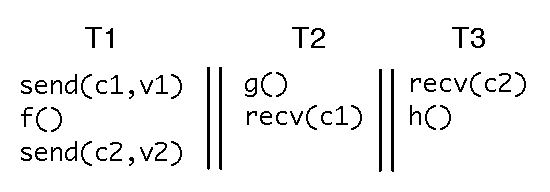
\includegraphics[scale=0.75]{Figures/IntroCode1}
\end{center}

\noindent Thread T1 performs a synchronous send on channel \cf{c1} that is
received by thread T2, after it computes \cf{g()}.  After the communication is
performed, T1 evaluates \cf{f()}, and then sends \cf{v2} on channel \cf{c2},
which is received by thread T3.  Upon receipt, T3 evaluates \cf{h()}. Assuming
\cf{f},\cf{g}, and \cf{h} perform no communication action of their own, the
synchronous communication on \cf{c1} by T1 could have been safely converted
into an asynchronous action in which \cf{v1} is buffered, and read by T2 later
upon evaluation of \cf{g()}.  The observable behavior of the program in both
cases (i.e., treating the initial send synchronously or asynchronously) would
be the same.

\begin{figure}[t]
\centering
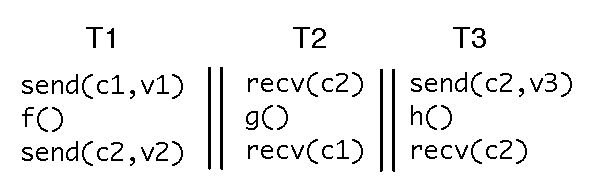
\includegraphics[scale=0.8]{Figures/IntroCode2}
\caption{Performing the first \cf{send} in T1 asynchronously is not meaning
preserving with respect to synchronous evaluation.}
\label{fig:intro2}
\end{figure}

Unfortunately, na\"{i}vely replacing synchronous communication with an
asynchronous one is not usually meaning-preserving as the example in
Figure~\ref{fig:intro2} illustrates. Under a synchronous evaluation protocol,
T2 would necessarily communicate first with T3, receiving \cf{v3} on channel
\cf{c2}.  It is then able to receive \cf{v1} from T1; finally, T1 can
communicate \cf{v2} to T3.  If the \cf{send(c1,v1)} operation by T1 were
replaced by \cf{asend(c1,v1)}, the first receive on T2 has, in addition to the
first send on T3, a \emph{new potential matching opportunity} -- the send of
\cf{v2} on channel \cf{c2}. If the receive by T2 matches with the send of
\cf{v2} on channel \cf{c2}, it is impossible to satisfy the send on T3. Thus,
this asynchronous execution exhibits a new behavior not possible using just
synchronous operators.

\begin{figure}[t]
\centering
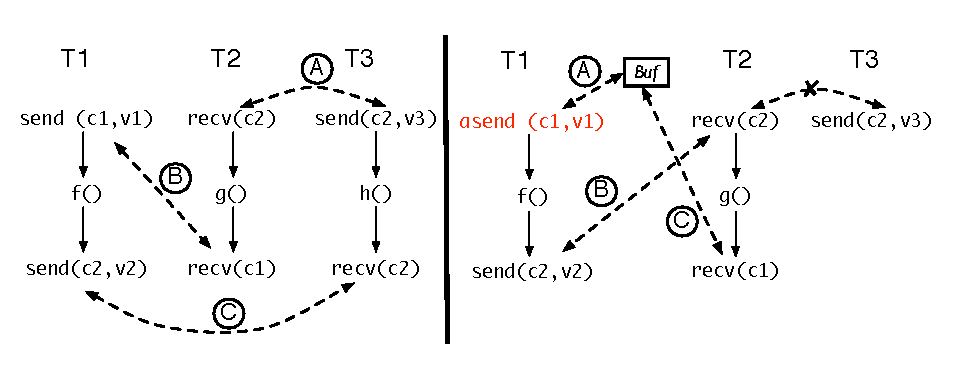
\includegraphics[scale=0.8]{Figures/IntroDepGraph}
\caption{Dependence graph induced by the execution of the program presented in Figure~\ref{fig:intro2}.}
\label{fig:dep_graph}
\end{figure}

The distinction between these two executions can be explained in terms of a
dependence graph that captures both intra- and inter-thread data- and
control-flow.  We can depict the executions by explicitly drawing these
dependencies as shown in Figure~\ref{fig:dep_graph}.

\noindent The dashed edges reflect communication and synchronization
dependencies among threads, while solid edges capture thread-local
control-flow. A bi-directional edge connects a sender with either a
receiver, in the case of a synchronous send, or a buffer, in the case where
it is asynchronous.  In both instances, there is a synchronization
dependence between endpoints, and a data dependence from the sender to
either the matching receiver or buffer.  The left-hand side of the figure
shows a possible execution in which all operations are synchronous; the
right considers an execution in which the initial send by T1 is
asynchronous.  The labels on the edges reflect the order in which
communication actions are executed.

\newcommand*\mycirc[1]{%
  \begin{tikzpicture}[baseline=(char.base)]
    \node[shape=circle,draw,inner sep=.3pt] (char) {#1};
  \end{tikzpicture}}

The synchronous execution on the left reflects the description given earlier.
The asynchronous execution on the right depicts the send on thread T1 buffering
its data (\mycirc{A}), thus allowing the synchronous communication between T1
and T2 (\mycirc{B}); this action prohibits communication between T2 and T3.  T2
subsequently receives \cf{v1} from the buffer associated with channel \cf{c1}
(\mycirc{C}).  This behavior could not be realized by any synchronous
execution: \mycirc{B} could never have been performed if the send operation on
channel \cf{c1} was not asynchronous.

The formalization of \emph{well-formed executions}, those that are the result
of asynchronous evaluation of CML send operations, but which nonetheless are
observably equivalent to a synchronous execution, and the means by which
erroneous executions, such as the right-hand execution above, can be detected
and repaired, form the focus of this chapter. Specifically, we make the
following contributions:

\begin{itemize}

\item We present the rationale for a \emph{relaxed execution model} for CML
that specifies the conditions under which a synchronous operation can be safely
executed asynchronously.  Our model allows applications to program with the
simplicity and composability of CML synchronous events, but reap the
performance benefits of implementing communication asynchronously.

\item We develop an axiomatic formulation of the model that can be used to
reason about correctness in terms of causal dependencies captured by a
\emph{happens-before} relation.  We relate this definition to an operational
semantics that specifies relaxed execution behavior for communicating actions,
and relate the set of traces admitted by the operational semantics to the safe
executions defined by the axiomatic formulation.

\item A distributed implementation, \rxcml, that treats asynchronous
communication as a form of \emph{speculation} is described. A mis-speculation,
namely the execution that could not have been realized using only synchronous
communication, is detected using a runtime instantiation of our axiomatic
formulation. An un-coordinated, distributed checkpointing mechanism is utilized
to rollback and re-execute the offending execution synchronously, which is
known to be safe.

\item Several case studies on a realistic cloud deployment demonstrate the
utility of the model in improving the performance of CML programs in
distributed environments without requiring \emph{any} restructuring of
application logic to deal with asynchrony.

\end{itemize}

\section{Motivation}

To motivate the utility of safe relaxation of synchronous behavior, consider
the problem of building a distributed chat application. The application
consists of a number of participants, each of whom can broadcast a message to
every other member in the group. The invariant that must be observed is that
any two messages sent by a participant must appear in the same order to all
members. Moreover, any message \cf{Y} broadcast in response to a previously
received message \cf{X} must always appear after message \cf{X} to every
member. Here, message \cf{Y} is said to be \emph{causally dependent} on
message \cf{X}.

\begin{figure}[t]
\begin{lstlisting}
datatype 'a bchan = BCHAN of ('a chan list (*val*) *
															unit chan list (*ack*))

(* Create a new broadcast channel *)
fun newBChan (n: int) (* n = number of participants *) =
  BCHAN(tabulate(n,fn _ => channel()), tabulate(n,fn _ => channel()))

(* Broadcast send operation *)
fun bsend (BCHAN (vcList, acList), v: 'a, id: int) : unit =
let
	val _ = map (fn vc => if (vc = nth (vcList, id)) then ()
												else send (vc, v))
						vcList (* phase 1 -- Value distribution *)
	val _ = map (fn ac => if (ac = nth (acList, id)) then ()
												else recv ac)
						acList (* phase 2 -- Acknowledgments *)
in ()
end

(* Broadcast receive operation *)
fun brecv (BCHAN (vcList, acList), id: int) : 'a=
let val v = recv (nth (vcList, id))
		val _ = send (nth (acList, id), ())
in v
end
\end{lstlisting}
\caption{Synchronous broadcast channel}
\label{code:bchan}
\end{figure}

Building such an application using a centralized server is straightforward, but
hinders scalability. In the absence of central mediation, a causal broadcast
protocol~\cite{Birman87} is required. One possible encoding of causal broadcast
using CML primitives is shown in Figure~\ref{code:bchan}. A broadcast operation
involves two phases.  In the first phase, values (i.e., messages) are
synchronously communicated to all receivers (except to the sender).  In the
second phase, the sender simulates a barrier by synchronously receiving
acknowledgments from all recipients.

The synchronous nature of the broadcast protocol along with the fact that the
acknowledgment phase occurs only after message distribution ensure that no
member can proceed immediately after receiving a message until all other
members have also received the message. This achieves the desired causal
ordering between broadcast messages since every member would have received a
message before the subsequent causally ordered message is generated. We can
build a distributed group chat server using the broadcast channel as shown
below.

\lstset{numbers=none}
\begin{lstlisting}
(* bc is broadcast chan, daemon is spawn as a separate thread *)
fun daemon id = display (brecv (bc, id)); daemon id
fun newMessage (m, id) = display m; bsend (bc, m, id)
\end{lstlisting}
\lstset{numbers=left,numberstyle=\tiny,stepnumber=1}

Assume that there are $n$ participants in the group, each with a unique
identifier \emph{id} between $0$ and $n-1$. Each participant runs a local
\emph{daemon} thread that waits for incoming messages on the broadcast channel
\cf{bc}. On a reception of a message, the daemon displays the message and
continues waiting. The clients broadcast a message using \cf{newMessage} after
displaying the message locally.  Observe that remote messages are only
displayed after all other participants have also received the message. In a
geo-distributed environment, where the communication latency is very high, this
protocol results in a poor user experience that degrades as the number of
participants increases.

Without making wholesale (ideally, zero!) changes to this relatively simple
protocol implementation, we would like to improve responsiveness, while
preserving correctness.  One obvious way of reducing latency overheads is to
convert the synchronous sends in {\tt bsend} to an asynchronous variant that
buffers the message, but does not synchronize with a matching receiver. There
are two opportunities where asynchrony could be introduced, either during value
distribution or during acknowledgment reception. Unfortunately, injecting
asynchrony at either point is not guaranteed to preserve causal ordering on the
semantics of the program.

\begin{figure}[t]
\begin{centering}
	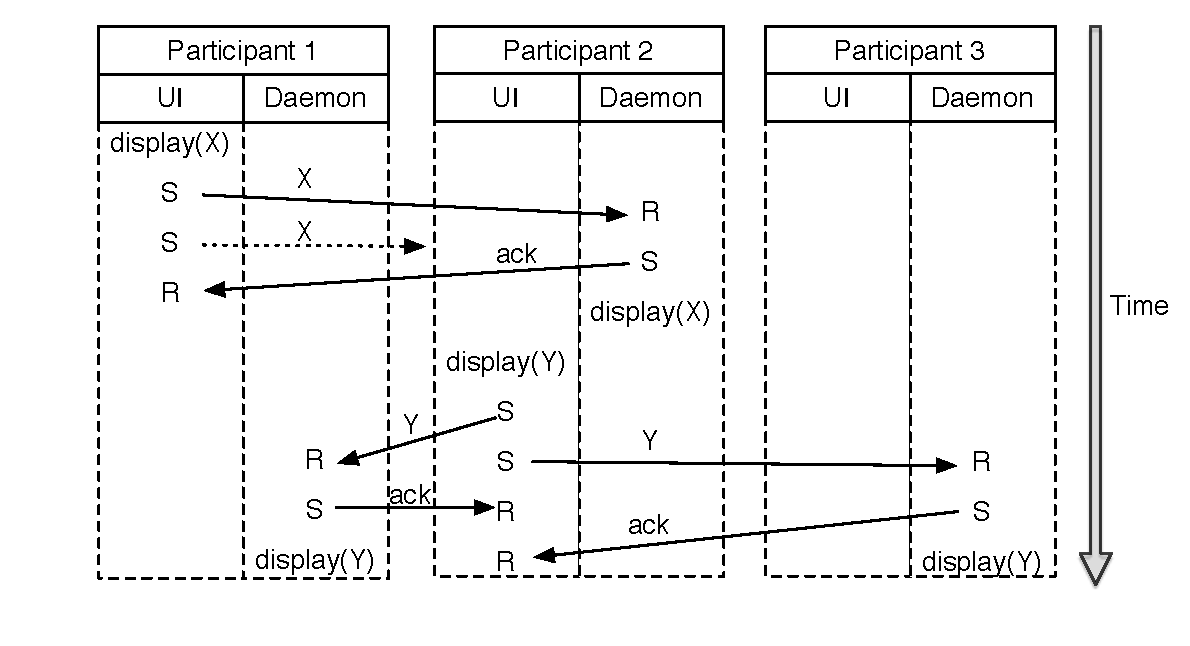
\includegraphics[width=0.8\textwidth] {Figures/ChatServer_AsyncValue}
	\caption{Incorrect execution due to unsafe relaxation of sends during
	broadcast. Dotted arrow represents in-flight message.}
	\label{fig:CS_asend_value}
\end{centering}
\end{figure}

Consider the case where the value is distributed asynchronously. Assume that
there are three participants: $p_1$, $p_2$, and $p_3$. Participant $p_1$ first
types message \cf{X}, which is seen by $p_2$, who in turn types the message
\cf{Y} after sending an acknowledgment. Since there is a causal order between
the message \cf{X} and \cf{Y}, $p_3$ must see \cf{X} followed by
\cf{Y}. Figure~\ref{fig:CS_asend_value} shows an execution where this is
not the case. In the figure, uninteresting messages have been elided for
clarity. The key observation is that, due to asynchrony, message \cf{X} sent
by the $p_1$ to $p_3$ might be \emph{in-flight}, while the causally dependent
message \cf{Y} sent by $p_2$ reaches $p_3$ out-of-order. This leads to a
violation of the protocol's invariants.

Similarly, it is easy to see that sending acknowledgments message
asynchronously is also incorrect. This would allow a participant that receives
a message to asynchronously send an acknowledgment, and proceed before all
other participants have received the same message. As a result, causal
dependence between messages is lost.

To quantify these issues in a realistic setting, we implemented a group chat
simulator application using a distributed extension of the MultiMLton Standard
ML compiler. We launched three Amazon EC2 instances, each simulating a
participant in the group chat application, with the same communication pattern
described in the discussion above. In order to capture the geo-distributed
nature of the application, participants were placed in three different
availability zones -- EU West (Ireland), US West (Oregon), and Asia Pacific
(Tokyo), resp.

During each run, $p_1$ broadcasts a message \cf{X}, followed by $p_2$
broadcasting \cf{Y}. We consider the run to be successful if the participant
$p_3$ sees the messages \cf{X},\cf{Y}, in that order.  The experiment was
repeated for 1K iterations. We record the time between protocol initiation and
the time at which each participant gets the message \cf{Y}. We consider the
largest of the times across the participants to be the running time. The
results are presented below.

\begin{center}
\begin{tabular}{ | l | r | r |}
	\hline
	\emph{Execution} 					& \emph{Avg.time (ms)} & \emph{Errors} \\
  \hline
	\emph{Sync}								& 1540	\ci{53} &	0 \ci{0} \\
	\emph{Unsafe Async} 			& 520		\ci{17} & 7 \ci{2} \\
	\emph{Safe Async (\rxcml)}	& 533		\ci{13} & 0 \ci{0} \\
  \hline
\end{tabular}
\end{center}

The \emph{Unsafe Async} row describes the variant where both value and
acknowledgment distribution is performed asynchronously; it is three times as
fast as the synchronous variant.  However, over the total set of 1K runs, it
produced seven erroneous executions. The \emph{Safe Async} row illustrates our
implementation, \rxcml, that detects erroneous executions on-the-fly and
remediates them. The results indicate that the cost of ensuring safe
asynchronous executions is quite low for this application, incurring only
roughly 2.5\% overhead above the unsafe version. Thus, in this application, we
can gain the performance benefits and responsiveness of the asynchronous
version, while retaining the simplicity of reasoning about program behavior
synchronously.

\section{Axiomatic Semantics}
\label{sec:axiomatic}

We introduce an axiomatic formalization for reasoning about the relaxed
behaviors of a concurrent message-passing programs with dynamic thread
creation. Not surprisingly, our formulation is similar in structure to
axiomatic formalizations used to describe, for example, relaxed memory
models~\cite{Demange2013,Sarkar2011,Sewell2010}.

An \emph{axiomatic execution} is captured by a set of \emph{actions} performed
by each thread and the relationship between them. These actions abstract the
relevant behaviors possible in a CML execution, relaxed or otherwise. Relation
between the actions as a result of sequential execution, communication, thread
creation and thread joins define the dependencies that any sensible execution must
respect. A relaxed execution, as a result of speculation, admits more behaviors
than observable under synchronous CML execution. Therefore, to understand the
validity of executions, we define a \emph{well-formedness} condition that
imposes additional constraints on executions to ensure their observable effects
correspond to correct CML behavior.

We assume a set of $\ThreadClass$ threads, $\ChannelClass$ channels, and
$\ValueClass$ values.  The set of actions is provided below. Superscripts $m$
and $n$ denote a unique identifier for the action.

\begin{mathpar}
\begin{array}{rcll}
\R{Actions} \; \ActionClass{}
	& \coloneqq & b_t 			& \R{(t starts)} \\
	& \mid      & e_t 			& \R{(t ends)} \\
	& \mid      & j_t^mt' 	& \R{(t detects t' has terminated)} \\
	& \mid      & f^m_tt' 	& \R{(t forks a new t')} \\
	& \mid 	    & s_t^mc,v 	& \R{(t sends value v on c)} \\
	& \mid      & r_t^mc   	& \R{(t receives a value v on c)} \\
	& \mid 	    & p_t^mv	 	& \R{(t outputs an observable value v)}
\end{array}

c      ~ \in ~ \ChannelClass ~ \R{(Channels)} \tab
t,t'   ~ \in ~ \ThreadClass ~ \R{(Threads)} \tab
v     ~ \in ~ \ValueClass ~ \R{(Values)} \tab
m,n ~ \in ~ \NumberClass ~ \R{(Numbers)}
\end{mathpar}

\noindent Action $b_t$ signals the initiation of a new thread with identifier
$t$; action $e_t$ indicates that thread $t$ has terminated.  A join action,
$j_t^mt'$, defines an action that recognizes the point where thread $t$ detects
that another thread $t'$ has completed.  A thread creation action, where thread
$t$ spawns a thread $t'$, is given by $f^m_tt'$. Action $s_t^mc,v$ denotes the
communication of data $v$ on channel $c$ by thread $t$, and $r_t^mc$ denotes
the receipt of data from channel $c$.  An external action (e.g., printing) that
emits value $v$ is denoted as $p_t^mv$.  We can generalize these individuals
actions into a family of related actions:
\begin{mathpar}
\begin{array}{lcll}
\ActionClass{r} &=& \{r_t^mc \mid t \in\ThreadClass\} & \R{(Receives)} \\
\ActionClass{s} &=& \{s_t^mc,v \mid t \in\ThreadClass, v\in\ValueClass\} & \R{(Sends)} \\
\ActionClass{c} &=& \ActionClass{s} \cup \ActionClass{r} & \R{(Communication)} \\
\ActionClass{o} &=& \{p_t^mv		 \mid	t \in\ThreadClass,v\in\ValueClass\} & \R{(Observables)} \\
\end{array}
\end{mathpar}

\noindent {\bf Notation.} We write $T(\alpha)$ to indicate the thread in which
action $\alpha$ occurs, and write $\,V(s_t^mc,v)$ to extract the value $v$
communicated by a send action. Given a set of actions $\ActionSet \in
2^\ActionClass{}$, $\ActionSet_x = \ActionSet \cap \ActionClass{x}$, where
$\ActionClass{x}$ represents one of the action classes defined above.

\begin{definition}[Axiomatic Execution]
\label{def:exec}
An axiomatic execution is defined by the tuple $\E \coloneqq \Exec$ where:
\begin{itemize}
\item $\program$ is a program.
\item $\ActionSet$ is a set of actions.
\item $\po \; \subseteq \ActionSet \times \ActionSet$ is the program order,
  a disjoint union of the sequential actions of each thread (which is a
  total order).
\item $\co \; \subseteq (\ActionSet_s \times \ActionSet_r) \cup (\ActionSet_r
	\times \ActionSet_s)$ is the communication order which is a symmetric
	relation established between matching communication actions (i.e., $\alpha
	\co \beta \implies \beta \co \alpha$). Moreover, a send and its matching
	receive must operate over the same channel (i.e., $s_t^mc,v \co r_{t'}^n{c'}
	\implies c = c'$).
\end{itemize}
\label{defn:exec}
\end{definition}

Additionally, there is an obvious ordering on thread creation and execution, as
well as the visibility of thread termination by other threads:

\begin{definition}[Thread Dependence]
\label{def:thr_dep}
If $\alpha = f_t^mt'$ and $\beta = b_{t'}$ or  $\alpha = e_t$ and $\beta = j_{t'}^mt$
then $\alpha \td \beta$ holds.
\end{definition}


\begin{definition}[Happens-before relation]
\label{def:hb}
The \textit{happens-before} order of an execution is the transitive closure of
the union of program order, thread dependence order, and actions related by
communication and program order:
\begin{mathpar}
\begin{array}{lll}
\hb & = & (\po \cup \td \cup \\
    &   &  \{ (\alpha,\beta)\ |\ \alpha \co \alpha' \wedge \alpha' \po \beta \}\ \cup \\
    &   &  \{ (\beta,\alpha)\ |\ \beta \po \alpha' \wedge \alpha' \co \alpha \})^+
\end{array}
\end{mathpar}
\end{definition}

\noindent For any two actions $\alpha,\beta \in \ActionSet$, if $\alpha \nbihb
\beta$, then $\alpha$ and $\beta$ are said to be \textit{concurrent} actions.
Importantly, our happens-before relation defines a preorder. A preorder is a
reflexive transitive binary relation. Unlike partial orders, preorders are not
necessarily anti-symmetric, i.e. they may contain cycles.

\begin{definition}[Happens-before Cycle]
A cycle exists in a happens-before relation if for any two actions
$\alpha, \beta$ and $\alpha \hb \beta \hb \alpha$.
\end{definition}

\lstset{numbers=none}
\begin{figure}[t]
\begin{lstlisting}
(* current thread is t1 *)
val t2 = spawn (fn () => recv c2; print "2"; recv c1)

val t3 = spawn (fn () => send(c2,v2); print "3"; recv c2)

val _ = send(c1,v1)
val _ = print "1"
val _ = send(c2,v2)
\end{lstlisting}
\caption{A CML Program with potential for mis-speculation.}
\label{code:simple}
\end{figure}
\lstset{numbers=left,numberstyle=\tiny,stepnumber=1,frame=single}

\begin{figure}[t]
\begin{minipage}{0.45\textwidth}
\subfigure[Well-formed execution]{\label{fig:well}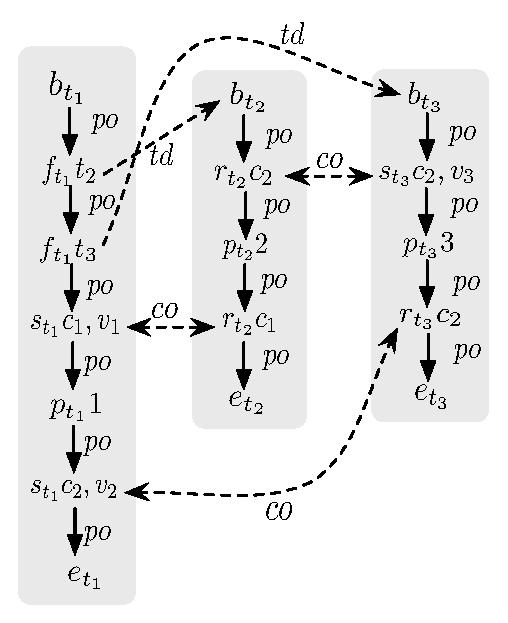
\includegraphics[width=1\textwidth]{Figures/AxiomaticExecution}}
\end{minipage}
\hfill
\begin{minipage}{0.45\textwidth}
\subfigure[Ill-formed execution]{\label{fig:ill}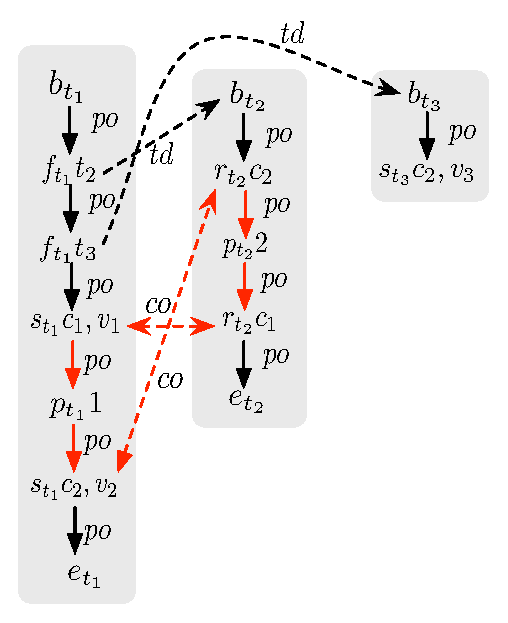
\includegraphics[width=1\textwidth]{Figures/AxiomaticExecution-1}}
\end{minipage}
\caption{Potential axiomatic executions of the CML program presented in Figure~\ref{code:simple}.}
\label{fig:pgm_and_execs}
\end{figure}

We provide an example to illustrate these definitions and to gain an insight
into erroneous executions that manifest as a result of speculative
communication. Consider the simple CML program (Figure~\ref{code:simple}) which
shows a simple CML program and two possible executions
(Figure~\ref{fig:pgm_and_execs}). The execution in Figure~\ref{fig:well}
imposes no causal dependence between the observable actions (i.e., print
statements) in $t_2$ or $t_3$; thus, an interleaving derived from this
execution may permute the order in which these statements execute. All
interleavings derivable from this execution correspond to valid CML behavior.

In contrast, the execution depicted in Figure~\ref{fig:ill}, exhibits a
happens-before cycle between $t_1$ and $t_2$, through a combination of program
and communication order edges. \emph{Such cyclic dependences never manifest in
any correct CML execution}. Cyclic dependences may however manifest when
synchronous sends are speculatively discharged asynchronously. We must
therefore strengthen our notion of correct executions to discard those that
contain such cycles.

To do so, we first note that the semantics as currently presented is concerned
only with actions that introduce some form of causal dependence either within a
thread (via program order) or across threads (via thread dependence or
communication order). However, a real program also does computation, and
reasoning about an execution's correctness will require us to specify these
actions as well. To facilitate this reasoning, we abstract the intra-thread
semantics, and parameterize our definition of an axiomatic execution accordingly.

\subsubsection{Intra-Thread Semantics.} The intra-thread semantics is abstracted
in our formulation via a labeled transition system.  Let $\intrastate$ denote
the intra-thread state of a thread; its specific structure is not interesting
for the purposes of the axiomatic definition. A labeled transition between
intra-thread states is captured by the relation, $\intratrans{.} \subseteq
\intrastate \times \intralabel \times \intrastate$, given to each thread $t \in
\ThreadClass$. The transition labels are in the set $\intralabel =
(\ActionClass{} \setminus \ActionClass{r}) \cup (\ActionClass{r} \times
\ValueClass) \cup \{\tau\}$.  Thus, a thread can either take a global action
step (e.g., creating another thread, performing a send action, ending a thread,
etc.), execute a \emph{silent} thread-local computation (denoted by label
$\tau$), or execute a receive action that receives the value associated with
the label. The requirements on the intra-thread semantics are:

\begin{itemize}
\item $\intratrans{.}$ can only relate states belonging to the same thread.
\item there is an initial state \ready: no transition leads to it,
	and a thread $t$ steps from it if and only if it emits a begin action $b_t$.
\item there is a final state \done: a thread leads to it if and only if it
	emits an end action $e_t$ and no transition leads from it.
\end{itemize}

\begin{definition}[Intra-trace]
\label{def:intra-trace}
Let $tr = \bar{\alpha}$ be a sequence of actions in set $\ActionSet$, and
$\co$ be a communication order on $\ActionSet$. Given a thread
$t \in \ThreadClass$ in a program $\program$, $tr$ is a valid intra-trace for
$t$ if there exists a set of states $\{\delta_0, \delta_1, \ldots \}$, and a
set of labels $\bar{l} = \{l_0, l_1,\ldots\}$ such that:
%
\begin{itemize}
\item for all $\alpha_i \in \bar{\alpha}, T(a) = t$
\item $\delta_0$ is the initial state \ready
\item for all $0 \leq i, \delta_{i} \intratrans{l_i} \delta_{i+1}$
\item the projection $\bar{\beta}$ of $\bar{l}$ to non-silent labels is such
	that $\beta_i = (\alpha_i, V(\gamma_i))$ if $\alpha_i \in \ActionSet_r$ and
	$\alpha_i \co \gamma_i$, or $\beta_i = \alpha_i$ otherwise.

\end{itemize}
\end{definition}

\noindent We write $\intraTraceSet[t]$ set of such pairs $(tr,\co)$ for
$\program$.

\begin{definition}[Well-formed Execution]
\label{def:well-formed}
An execution $E \coloneqq \Exec$ is well-formed if the following
conditions hold:
%
\begin{enumerate}
\item Intra-thread consistency: for all threads $t \in \ThreadClass,
	\;(\restrict{\po}{t}, \co) \in \intraTraceSet[t]$
\item Happens-before correctness: The happens-before relation $\hb$ constructed
	from $E$ has no cycles.
\item Observable correctness: Given $\alpha  \in \ActionSet_{o}$ and  $\beta
	\in \ActionSet_{c}$ if $\beta \hb \alpha$ then there exists $\beta' \in
	\ActionSet_{c}$ s.t. $\beta \co \beta'$.
\end{enumerate}
\end{definition}

For an axiomatic execution $\E \coloneqq \Exec$ to be well-formed, the actions,
program order and communication order relations must have been obtained from a
valid execution of the program $\program$ as given by the intra-thread
semantics defined above (1). As we noted in our discussion of
Figure~\ref{fig:pgm_and_execs}, no valid execution of a CML program may involve
a cyclic dependence between actions; such dependencies can only occur because
of \emph{speculatively} performing what is presumed to be a synchronous send
operation (2).

Finally, although the relaxed execution might speculate, i.e., have a send
operation transparently execute asynchronously, the observable behavior of such
an execution should mirror some valid non-speculative execution, i.e., an
execution in which the send action was, in fact, performed synchronously.  We
limit the scope of speculative actions by requiring that they complete (i.e.,
have a matching recipient) before an observable action is performed (3).
Conversely, this allows communication actions not preceding an observable
action to be speculated upon. Concretely, a send not preceding an externally
visible action can be discharged asynchronously. The match and validity of the
send needs to be checked only before discharging the next such action. This is
the key idea behind our speculative execution framework.

\subsubsection{Safety.} An axiomatic execution represents a set
of interleavings, each interleaving defining a specific total order that is
consistent with the partial order defined by the execution\footnote{Two
ordering relations $P$ and $Q$ are said to be \textit{consistent} if
$\forall x,y, \neg(xPy \conj yQx)$.}.  The well-formedness conditions of an
axiomatic execution implies that any observable behavior of an interleaving
induced from it must correspond to a synchronous CML execution. The
following two definitions formalize this intuition.

\begin{definition}[Observable dependencies]
\label{def:od}
In a well-formed axiomatic execution $\E \coloneqq \Exec$, the observable
dependencies $\ActionSet_{od}$ is the set of actions that precedes (under
$\hb$) some observable action, i.e., $\ActionSet_{od} = \{\alpha \ALT \alpha \in
\ActionSet, \beta \in \ActionSet_{o}, \alpha \hb \beta\}$.
\end{definition}

\begin{definition}[$\cml$ Execution]
\label{def:cml}
Given a well-formed axiomatic execution $\E \coloneqq \Exec$, the pair $(\E,
\toto)$ is said to be in $\cml(\program)$ if $\toto$ is a total order on
$\ActionSet_{od}$ and $\toto$ is consistent with $\hb$.
\end{definition}

In the above definition, an interleaving represented by $\toto$ is only possible
since the axiomatic execution is well-formed, and thereby does not contain a
happens-before cycle.

\begin{lemma}
\label{lem:toto_hb}
If a total order $\toto$ is consistent with $\hb$, then $\hb$ does not contain
a cycle involving actions in $\ActionSet_{od}$.
\end{lemma}

Next, we show that a well-formed axiomatic execution respects the safety
property of a CML program executed non-speculatively. When a CML program
evaluates non-speculatively, a thread performing a communication action is
blocked until a matching communication action is available. Hence, if
$(\Exec,\toto) \in \cml(\program)$, and a communication action $\alpha$ on a
thread $t$ is followed by an action $\beta$ on the same thread, then it must be
the case that there is a matching action $\alpha \co \alpha'$ that happened
before $\beta$ in $\toto$. This is captured in the following theorem.

\begin{theorem}
Given a CML execution $(\E, \toto) \in \cml(\program)$, $\forall \alpha,\beta$
such that $\alpha \in \ActionClass{c}, T(\alpha) = T(\beta), \alpha \toto \beta$,
there exists an action $\alpha \co \alpha'$ such that $\alpha' \toto
\beta$.
\end{theorem}
\begin{proof}
Let $\E \coloneqq \Exec$. First, we show that $\alpha' \in \ActionSet$. Since
$\alpha \toto \beta$, $\alpha \in \ActionSet_{od}$, by
Definition~\ref{def:cml}. By Definition~\ref{def:od}, there exists some $\gamma
\in \ActionSet_o$ such that $\alpha \hb \gamma$. Since $\E$ is well-formed and
$\alpha \hb \gamma$, by Definition~\ref{def:well-formed}, there exists an
$\alpha' \in \ActionSet$ such that $\alpha \co \alpha'$.

Next, we show that $\alpha' \in \ActionSet_{od}$. By Definition~\ref{def:hb},
$\alpha' \co \alpha \hb \gamma$ implies $\alpha' \hb \gamma$. Hence, $\alpha'
\in \ActionSet_{od}$, and is related by $\toto$. Finally, since $T(\alpha) =
T(\beta)$ and $\alpha \toto \beta$, $\alpha \po \beta$. And, $\alpha' \co
\alpha \po \beta$ implies $\alpha' \hb \beta$. By Lemma~\ref{lem:toto_hb} and
Definition~\ref{def:cml}, $\alpha' \toto \beta$.
\end{proof}

\section{Operational Semantics}

\begin{figure}[t]
\begin{minipage}[t]{\columnwidth}
\begin{smathpar}
\begin{array}{lclcl}
e & \in & {\tt Exp} & := 		& v \ALT x \ALT e \; e \ALT \chan() \ALT \print(e) \ALT \spawn(e) \\
	&			&						& \ALT 	&	\send(e,e) \ALT 	\recv(e) \ALT \join(e)\\
v & \in & {\tt Val} & := 		& \unit \ALT c \ALT \lambda\,x.e \ALT t \\
\end{array}
\end{smathpar}
\end{minipage}
%
\begin{minipage}[t]{\columnwidth}
\begin{smathpar}
\begin{array}{lcl}
E & := 		& \bullet \ALT E\;e \ALT v\;E \ALT \print(E) \\
  & \ALT 	& \spawn(E) \ALT \send(E,e) \ALT \send(c,E) \\
	& \ALT	& \recv(E) \ALT \join(E)
\end{array}
\end{smathpar}
\end{minipage}

\begin{minipage}[t]{\columnwidth}
\begin{smathpar}
\begin{array}{lclcl}
c & \in & {\tt ChannelId}\\
\alpha,\beta 	& \in & {\tt Action} & := & \ActionClass\ \ALT (\alpha,\beta) \ALT\ \tau_t \ALT \commit{\program}{\trace}\\
\ActionSoup 	& \in & {\tt SendSoup}		& := & \ActionClass{s}\\
\localstate 	& \in & {\tt LocalState} & := & e \ALT \readyOp{e} \ALT \doneOp \\
t 						& \in & {\tt ThreadId}\\
\thread 			& \in & {\tt Thread} 				& := & (t,\localstate) \\
\threadsoup 	& \in & {\tt ThreadSoup}		& := & \emptyset \ALT \thread \;\|\; \threadsoup\\
\langle \threadsoup,\ActionSoup \rangle	& \in & \ProgramState
\end{array}
\end{smathpar}
\end{minipage}
\caption{Syntax and states for the relaxed execution semantics of a subset of CML.}
\label{sem:rxcml_op_syntax}
\end{figure}

\begin{figure}[t]
\begin{smathpar}
\begin{array}{cl}

\RULEONE
{\PrgState{(\lambda\,x.e) v}{\ActionSoup}
\intertrans{\tau_t}
\PrgState{e[v/x]}{\ActionSoup}} & \rulelabel{App} \\ \\

\RULE
{c \;\; \fresh \;\;\; }
{\PrgState{\chan()}{\ActionSoup}
\intertrans{\tau_t}
\PrgState{c}{\ActionSoup}} & \rulelabel{Chan} \\ \\

\RULEONE
{\langle (t,\readyOp{e}) \;\|\; \threadsoup, \ActionSoup \rangle
 \intertrans{b_t}
 \langle (t,e) \;\|\; \threadsoup, \ActionSoup \rangle} & \rulelabel{Begin} \\ \\

\RULEONE
{\langle (t,v) \;\|\; \threadsoup,\ActionSoup \rangle
 \intertrans{e_t}
 \langle (t,\doneOp) \;\|\; \threadsoup, \ActionSoup \rangle} & \rulelabel{End} \\ \\

\RULEONE
{\PrgState{\spawn\,e}{\ActionSoup}
\intertrans{f_t^it'}
\langle (t,\opIntraState{t'}) \;\|\; (t',\readyOp{e}) \;\|\; \threadsoup, \ActionSoup \rangle} & \rulelabel{Spawn} \\ \\

\RULEONE
{\langle (t,\opIntraState{\join\,t'}) \;\|\; (t',\doneOp) \;\|\; \threadsoup, \ActionSoup \rangle
 \intertrans{j_t^it'}
 \langle (t,\opIntraState{\unit}) \;\|\; (t',\doneOp) \;\|\; \threadsoup, \ActionSoup \rangle} & \rulelabel{Join} \\ \\

\RULEONE
{\PrgState{\print\,v}{\ActionSoup} \intertrans{p_t^iv}
\PrgState{\unit}{\ActionSoup}} & \rulelabel{Print} \\ \\

\RULE
{\alpha = s_t^ic,v}
{\PrgState{\send(c,v)}{\ActionSoup}
 \intertrans{\alpha}
 \PrgState{\unit}{\ActionSoup \cup \{\alpha\}}} & \rulelabel{Send} \\ \\

\RULE
{\alpha = r_t^ic \;\;\; \beta = (s_{t'}^jc,v) \in \ActionSoup}
{\PrgState{\recv\,c}{\ActionSoup}
\intertrans{(\alpha,\beta)}
\PrgState{v}{\ActionSoup \setminus \beta}} & \rulelabel{Recv} \\ \\

\RULE
{\wf{(\program,\trace)}}
{\langle\threadsoup,\ActionSoup\rangle
\intertrans{\commit{\program}{\trace}}
\langle\threadsoup,\ActionSoup\rangle} & \rulelabel{Commit}

\end{array}
\end{smathpar}
\caption{A relaxed execution operational semantics for a subset of CML.}
\label{fig:op_semantics}
\end{figure}

The axiomatic semantics provides a declarative way of reasoning about
executions. However, it is unclear how to use this semantics to
\emph{execute} a CML program that performs the sends asynchronously
while ensuring that the observable behaviors correspond to a
synchronous execution of the program; that is, how we can we ensure
that implementations produce relaxed executions that always conform to
a CML execution in the sense of Definition~\ref{def:cml}?  In this
section, we present an operational definition of a relaxed execution
as a labeled transition system that allows us to express the
constraints necessary to prevent non-CML observable behaviors.

The operational machine, $\rel$, takes as its input an operational execution,
which is composed of a program, and a trace $\trace$ of \emph{operational
actions}. It evaluates the program according to the trace, by manipulating a
\emph{send soup}, an unordered set into which pending sends are added
asynchronously.  Informally, we can think of the trace as a history or log of
actions we wish to perform; the machine either accepts the trace, if executing
the actions found in the trace using the reduction rules leads to a CML
execution (as defined by Definition~\ref{def:cml}), or gets stuck otherwise.

\begin{definition}[Operational Action]
\label{def:op_act}
An operational action $\alpha \in \ActionClass{op}$ is either:

\begin{itemize}
\item an action in $\ActionClass{} \setminus \ActionClass{r}$.
\item a pair in $\ActionClass{r} \times \ActionClass{s}$ where each receive
	action is paired up with the matching send action on the same channel,
\item a \emph{silent} action $\tau_t$ indexed by a thread identifier that
  indicates the evaluation of a computation step (e.g., a function call).
\item a \emph{commit} action $\commit{\program}{\trace}$ that checks whether
  the machine state is well-formed in the sense of
  Definition~\ref{def:well-formed}.  Intuitively, a well-formed machine
  state is one that could have been reached if all \cf{send} operations
  were executed synchronously.
\end{itemize}
\end{definition}

\begin{definition}[Operational Execution]
An operational execution is a pair $(\program,tr)$, where $\program$ is a
program and $tr \in \bar{\ActionClass{op}}$, and there are no duplicates in
$tr$.
\end{definition}

The operational semantics of the machine used to interpret the trace is given
in Figure~\ref{sem:rxcml_op_syntax} and Figure~\ref{fig:op_semantics}.  The
program state is composed of a tuple with $\threadsoup$ representing the pool
of concurrently executing threads and a collection of unmatched send actions
$\ActionSoup$. Each thread in $\threadsoup$ is a tuple with a thread id and a
local state.  This state is either an initial state $\readyOp{e}$ containing
the expression that will be evaluated by this thread, or a completed state
$\doneOp$, or the expression being evaluated by this thread.  Each state
transition is affixed with an action drawn from the trace that is used by the
machine to determine which rule to apply, as we describe below.

The source language contains function abstraction, application, first-class
channels, a thread creation operation ({\sf spawn}), message-passing
primitives on these channels, and a {\sf print} statement to capture an
observable action.  Reductions are labeled with operational actions. Rules
{\sc App} and {\sc Chan} represent silent (thread-local) actions.  The {\sc
  Spawn} rule creates a new thread with the initial local state
$\readyOp{e}$. Rule {\sc Begin} initiates execution of the thread from its
initial state.  A thread moves to the $\doneOp$ local state once the
expression being evaluated is reduced to a value (Rule {\sc End}). The
completed thread remains in the thread pool so that other threads may also
join on it.  A thread can wait on another thread's completion by joining on
its thread identifier. The calling thread is paused until the joined thread
moves to the final local state $\doneOp$ (Rule {\sc Join}).

The {\sc Send} rule adds the associated send action $\alpha$ into
$\ActionSoup$, the collection of pending send actions, and allows execution to
proceed.  Thus, this rule captures asynchronous behavior. The transition
defined by the {\sc Recv} has a label defined as a pair, consisting of the
receive action $\alpha$ and an unmatched send action $\beta$, which belongs to
the send pool. The receiver thread consumes the value contained in the send
action, and removes the action from $\ActionSoup$.  An observable action (rule
{\sc Print}) is evaluated only if the trace emits a print action; this rule
exists primarily to allow us to reason about equivalence of observable
behaviors as we describe below.  Finally, we define a commit rule (rule {\sc
Commit}) that checks whether the interleaving generated thus far corresponds to
a sensible CML execution, i.e., whether the interleaving exhibits a behavior
that could have been observed if all \cf{send} operations executed thus far
were evaluated synchronously. It uses an operator {\sf WF} defined in
definition~\ref{def:well-formed-rel}.

\begin{definition}[$\rel$ execution]

Given a trace $\trace = \bar{\beta}.\commit{\program}{\bar{\beta}}$
terminating in a commit action, an operational execution $(\program,
\trace)$ is a \emph{relaxed} execution ($\rel(\program,\trace)$) if there
exists an ordered sequence $\bar{\delta} \in \ProgramState$ satisfying the
following:

\begin{itemize}
\item $\delta_0 = \langle (t_0,\readyOp{\program}),\emptyset\rangle$ for some
unique thread identifier $t_0$.
\item for all $\alpha_i \in \trace$, there exists $\delta_{i}$,
  $\delta_{i+1} \in \bar{\delta}$ such that $\delta_{i} \intertrans{\alpha_i}
  \delta_{i+1}$.
\end{itemize}
\end{definition}

\noindent Clearly, not every operational execution $(\program,\mathit{tr})$ is a
relaxed execution.  Consider the following program $\program$:

\begin{center}
\begin{lstlisting}
fun main () =
let val c = channel()
in print (send(c,v); recv c)
end
\end{lstlisting}
\end{center}

\noindent with trace
  \[ \trace = b_t~.~s_t^ic,v~.~(r_t^jc;\;s_t^ic,v)~.~p_t^kv~.~e_t \]

\noindent where silent transitions have been elided.  When suffixed with a
commit action $\commit{\program}{\trace}$, the resulting behavior would not be
accepted by the semantics, since no synchronous execution of the program would
result in a match of the \cf{send} operation with a \cf{recv} action on the
same thread.  The prohibition of such behavior is encapsulated within the
definition of well-formedness found in the antecedent of the {\sc Commit} rule
that we formalize below.

We reason about sensible (well-formed) relaxed executions by transforming them
into an equivalent axiomatic one.  A well-formed $\rel$ execution is one whose
corresponding axiomatic execution is well-formed. Since an axiomatic semantics
is parameterized by an intra-thread semantics, we first provide a translation
that produces this semantics given the transitions defined by the operational
semantics.

\begin{definition}[Intra-thread semantics]
\label{def:intra-rel}
Given a program $\program$, let
\[\intrastate \coloneqq \ready \ALT \done \ALT e\]
where $e \in \program$. For each labeled transition of the form $\langle
(t,s) \| \threadsoup, \ActionSoup \rangle \intertrans{\alpha} \langle (t,s') \|
\threadsoup', \ActionSoup' \rangle$, where $\alpha \neq
\commit{\program}{\trace}$, we define $\delta \intratrans{\beta} \delta'$,
where $\delta, \delta' \in \intrastate$ such that:
\begin{itemize}
	\item if $s = \readyOp{e}$, then $\delta = \ready$, otherwise, $\delta = s$.
	\item if $s' = \doneOp$, then $\delta' = \done$, otherwise $\delta' = s'$
	\item if $\alpha = ((r_t^ic),\,(s_{t'}^jc,v))$ then $\beta = (r_t^ic;\,v)$
  \item if $\alpha = \tau_t$ then $\beta = \tau$
  \item otherwise, $\alpha = \beta$
\end{itemize}

\end{definition}

\begin{definition}[$\opax$ operator]
\label{def:opax}
Let $\E_{o} = (\program, tr)$ be an operational execution. $\opax$ is defined
as $\opax(\E_{o}) = \Exec$ parameterized with the intra-thread semantics
$\intratrans{}$ (Definition~\ref{def:intra-rel}), where

\begin{itemize}
\item $\ActionSet$ is a set of non-silent, non-commit actions in $tr$.
\item for all $\alpha,\beta \in \ActionSet$, $\alpha \po \beta$ iff $T(\alpha)
	= T(\beta)$ and $\alpha$ precedes $\beta$ in $tr$.
\item for all pairs $(a,b)$ such that $a = r_t^ic$ and $b = s_{t'}^jc,v$, $a
	\co b \wedge b \co a$
\end{itemize}
\end{definition}

For perspicuity, in the definition of $\ActionSet$ and $\po$ above, a receive
operational action $(a,b) \in \ActionClass{op}$ is simply treated as $a \in
\ActionClass{r}$.

\begin{definition}[Well-formed $\rel$ execution]
\label{def:well-formed-rel}
Let $\E_o = (\program,tr) \in \rel(\program)$ be an operational execution. If
the axiomatic execution $\E_{ax} = \opax(\E_o)$ is well-formed, then $\E_o$ is
well-formed. This is written as $\wf{\E_o}$.
\end{definition}

\begin{theorem}
If $E_o = (\program,\trace)$ and $\wf{E_o}$, then \mbox{$(\opax(\E_o), \toto) \in
\cml(\program)$}.
\end{theorem}

\begin{proof}
We provide a witness for $\opax(\E_o)$ via a generative operator $\opaxGen$
(Definition~\ref{def:opaxGen}) such that $\opaxGen(\E_o)$ is an axiomatic
execution (Theorem~\ref{thm:g_ax}) and $\opaxGen(\E_o) = \opax(\E_o)$
(Theorem~\ref{thm:g_eq_t}). We then prove that if $\E_o$ is well-formed, then
$\opaxGen(\E_o)$ is well-formed (Lemma~\ref{lem:wf_opaxGen}). Since
$\opaxGen(\E_o)$ is well-formed, by definition~\ref{def:cml} and
theorem~\ref{thm:g_eq_t}, $(\opax(\E_o), \toto) \in \cml(\program)$.
\end{proof}

\begin{definition}[$\opaxGen$ operator]
\label{def:opaxGen}
Let $\E_{op} = (\program,\trace) \in \rel(\program)$ be a well-formed
operational execution. $\opaxGen(\E_{op})$ is an axiomatic execution
parameterized with the intra-thread semantics $\intratrans{}$
(definition~\ref{def:intra-rel}) defined as follows:
\begin{itemize}
\item $\opaxGen(\program,\emptyset) = \langle \program, \emptyset, \emptyset,
	\emptyset \rangle$
\item If $\opaxGen(\program,\bar{\alpha}) = \Exec$ , then $\E_{ax} =
	\opaxGen(\program,\bar{\alpha}.\beta)$ defined as follows:
	\begin{enumerate}
	\item if $\beta = \tau_t$ or $\beta = \commit{\program}{\bar{\alpha}}$, then
		$\E_{ax} = \Exec$
	\item if $\beta \notin (\ActionClass{r} \times \ActionClass{s})$, then $\E_{ax} =
		\langle \program, \ActionSet \cup \{\beta\}, \po \cup~ \{\gamma \po \beta \ALT
		\gamma \in \ActionSet, T(\gamma) = T(\beta)\}, \co \rangle$
	\item if $\beta = (\gamma,\,\zeta)$, then $\E_{ax} = \langle \program,
		\ActionSet \cup \{\gamma\}, \po \cup~ \{\eta \po \gamma \ALT \eta \in
		\ActionSet, T(\eta) = T(\gamma)\}, \co \cup~ \{\gamma \co \zeta, \zeta \co
		\gamma\} \rangle$
	\end{enumerate}
\end{itemize}
\end{definition}

\begin{theorem}
\label{thm:g_ax}
Let $\E_{op} = (\program,\trace) \in \rel(\program)$ be an operational
execution. Then, $\opaxGen(\E_{op})$ is an axiomatic execution.
\end{theorem}
\begin{proof}
We show that the quadruple generated by the $\opaxGen$ operator satisfies the
conditions necessary for an axiomatic execution (Definition~\ref{def:exec}). In
particular, (1) $\ActionSet$ is composed of actions from $\ActionClass{}$, (2)
$\po$ is a disjoint total order on actions belonging to each thread. (3) $\co$
is a symmetric relation and relates actions belonging to the same channel. We
show these conditions hold by induction on $\left|{\trace}\right|$.

The base case is if $\E_{op} = (\program,\emptyset) \in \rel(\program)$, then
$\opaxGen(\E_{op})$ is an axiomatic execution. If the trace is empty, then
$\opaxGen(\E_{op}) = \Exec$. Here, $\program$ is a valid program. $\ActionSet$,
$\po$, and $\co$ are empty. Hence, the conditions defined under
Definition~\ref{def:exec} trivially hold.

Assume $\opaxGen(\program,\bar{a})$ is an axiomatic execution.  We show that
$\opaxGen(\program,\bar{a}.b)$ is an axiomatic execution, where $b \in
\ActionClass{op}$. If $b$ is a silent action or a commit action
(Definition~\ref{def:opaxGen}.1), then $\opaxGen(\program,\bar{a}.b) =
\opaxGen(\program,\bar{a})$.

Let $b \notin (\ActionClass{r} \times \ActionClass{s})$. Then $b \in
\ActionClass{}$ (Definition~\ref{def:op_act}). In this case
(Definition~\ref{def:opaxGen}.2), $\opaxGen$ operator adds $b$ to $\ActionSet$
and adds $\po$ edges from all actions $\alpha \in \ActionSet$ such that
$T(\alpha) = T(b)$ to $b$ (preserving the total order). $\co$ is not modified.
By the induction hypothesis, $\opaxGen(\program,\bar{a}.b)$ is an axiomatic
execution.

Let $b = (\alpha,\beta)$. $\alpha \in \ActionClass{r}, \beta \in
\ActionClass{s}$ (Definition~\ref{def:op_act}).   In this case, by
Definition~\ref{def:opaxGen}.3, $\opaxGen$  adds $\alpha$ to $\ActionSet$, and
introduces $\po$ edges from all actions in $\ActionSet$ that belong to the
thread $T(\alpha)$ to $\alpha$ (preserving the total order). $\co$ is extended
with $\{\alpha \co \beta, \beta \co \alpha\}$. By the induction hypothesis,
$\co$ is a symmetric relation. By Definition~\ref{def:op_act}, $\alpha$ and
$\beta$ operate on the same channel. Thus, $\opaxGen(\program,\bar{a}.b)$ is an
axiomatic execution.
\end{proof}

\begin{theorem}
\label{thm:g_eq_t}
Given $\E_o = (\program,\trace) \in \rel(\program)$, $\opax(\E_o) =
\opaxGen(\E_o)$.
\end{theorem}
\begin{proof}
By theorem~\ref{thm:g_ax}, $\opaxGen(\E_o)$ is an axiomatic execution. We need
to show that each component in the axiomatic execution defined by $\opax$ and
generated by $\opaxGen$ are the same.  Both operators use the same program
$\program$ and set of actions $\ActionSet$ from $\E_o$.

$\opax$ defines a $\po$ relation between actions $\alpha$ and $\beta$ iff
$T(\alpha) = T(\beta)$ and $\alpha$ precedes $\beta$ in the trace
(Definition~\ref{def:opax}.1).  Assume that the operational trace is
$\trace = \bar{\alpha}.\beta$.  For any $\gamma$ such that $T(\gamma) =
T(\beta)$, $\gamma \in \bar{\alpha}$, $\gamma$ belongs to the action set
$\ActionSet$ of
$\opaxGen(\program,\bar{\alpha})$. Definition~\ref{def:opaxGen}.2 and
\ref{def:opaxGen}.3 add a $\po$ edge from such a $\gamma$ to $\beta$.

Definition~\ref{def:opax}.3 defines $\co$ such that for all pairs
$(\alpha,\beta)$ in \emph{tr}, $\alpha \co \beta$ and $\beta \co \alpha$.
$\opaxGen$ extends $\co$ in a similar fashion
(Definition~\ref{def:opaxGen}.3).
\end{proof}

\begin{lemma}
\label{lem:wf_opaxGen}
Let $\E_o = (\program,\trace) \in \rel(\program)$. If $\E_o$ is well-formed,
then $\opaxGen(\E_o)$ is well-formed.
\end{lemma}
\begin{proof}
Since $\E_o$ is well-formed, $\opax(\E_o)$ is a well-formed axiomatic execution
(by Definition~\ref{def:well-formed-rel}). By Theorem~\ref{thm:g_eq_t},
$\opax(\E_o) = \opaxGen(\E_o)$. Hence, $\opaxGen(\E_o)$ is a well-formed
axiomatic execution.
\end{proof}

\section{Implementation}
\label{sec:implementation}

The axiomatic semantics provides a declarative way of reasoning about correct
CML executions. In particular, a well-formed execution does not have a
happens-before cycle. However, in practice, a speculative execution framework
that discharges synchronous sends asynchronously (speculatively), needs to
track the relations necessary to perform the integrity check \emph{on-the-fly},
detect and remediate any execution that has a happens-before cycle.

To do so, we construct a \emph{dependence graph} that captures the dependencies
described by an axiomatic execution, and ensure the graph has no cycles. If a
cycle is detected, we rollback the effects induced by the offending speculative
action, and re-execute it as a normal synchronous operation. By definition,
this synchronous re-execution is bound to be correct. The context of our
investigation is a distributed implementation of CML called \rxcml ({\sc
RelaXed CML}) built on top of the MultiMLton SML compiler and
runtime~\cite{JFP14}. We have extended MultiMLton with the infrastructure
necessary for distributed execution.

\subsection {System Architecture}

\begin{figure}[t]
\centering
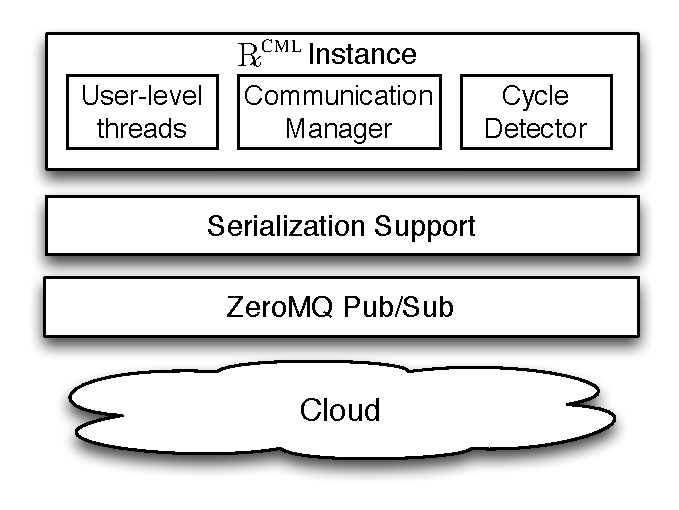
\includegraphics[width=0.5\textwidth]{Figures/CRexDesign}
\caption{\rxcml application stack.}
\label{fig:c-rex}
\end{figure}

A schematic diagram of the \rxcml application stack is presented in
Figure~\ref{fig:c-rex}. An \rxcml application consists of multiple
\emph{instances}, each of which runs the \emph{same} MultiMLton executable.
These instances might run on the same node, on different nodes within the same
datacenter, or on nodes found in different data centers. Each instance has a
scheduler which preemptively multiplexes execution of user-level CML threads
over multiple cores. We use the ZeroMQ messaging library~\cite{zeromq} as the
transport layer over which the \rxcml channel communication is implemented. In
addition to providing reliable and efficient point-to-point communication,
ZeroMQ also provides the ability to construct higher-level multicast patterns.
In particular, we leverage ZeroMQ's publish/subscribe support to implement
CML's first-class channel based communication.

The fact that every instance in an \rxcml application runs the same program, in
addition to the property that CML channels are strongly-typed, allows us to
provide typesafe serialization of immutable values as well as function
closures. Serializing mutable references is disallowed, and an exception is
raised if the value being serialized refers to a mutable object. To safely
refer to the same channel object across multiple instances, channel creation is
parameterized with an identity string. Channels created with the same identity
string refer to the same channel object across all instances in the \rxcml\
application. Channels are first-class citizens and can be sent as messages over
other channels to construct complex communication protocols.

\subsection{Communication Manager}
\label{sec:comm_mgr}

Each \rxcml instance runs a single communication manager thread, which
maintains globally consistent replica of the CML channels utilized by its
constituent CML threads. The protocol for a single CML communication is
illustrated in Figure~\ref{fig:comm_mgr}. Since CML channel might potentially
be shared among multiple threads across different instances, communication
matches are determined dynamically. In general, it is not possible to determine
the matching thread and its instance while initiating the communication action.
Hence, whenever a thread intends to send or receive a value on the channel, its
intention (along with a value in the case of a send operation), is broadcast to
every other \rxcml instance. Importantly, the application thread performing the
send does not block and \emph{speculatively} continues execution.

\begin{figure}[t]
\centering
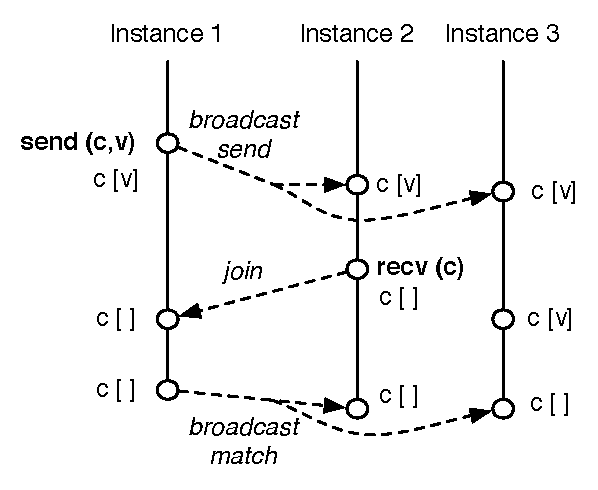
\includegraphics[width=0.55\textwidth]{Figures/CommunicationManager}
\caption{Communication manager behavior during a send and its matching receive.}
\label{fig:comm_mgr}
\end{figure}

Subsequently, an application thread that performs a receive on this channel
consumes the send action, sends a \emph{join message} to the sender thread's
instance, and proceeds immediately. In particular, receiver thread does not
block to determine if the send action was concurrently consumed by a thread in
another instance. This corresponds to speculating on the communication match,
which will succeed in the absence of concurrent receives for the same send
action. On receiving the join message, a \emph{match message} is broadcast to
every instance, sealing the match. Those instances that speculatively matched
with the send, except the one indicated in the match message, treat their
receive action as a mis-speculation. Other instances that have not matched with
this particular send remove the send action from the corresponding local
channel replica.

\subsection{Speculative Execution}

Aborting a mis-speculation requires restoring the computation to a previously
known consistent state. Achieving this entails rolling back all threads that
communicated with the offending action, transitively. In this regard,
\emph{stabilizers}~\cite{Ziarek10} provide a suitable abstraction for restoring
consistent checkpoints in message-passing programs.  A stabilizer builds a
dependence graph that takes into account intra-thread program order and
inter-thread communication dependence. However, the implementation reported
in~\cite{Ziarek10} assumes a centralized structure, and a global barrier that
stops all execution while a checkpoint is restored; neither condition is
reasonable in a high-latency, distributed environment.

\subsubsection{Replicated Dependence Graph.} Instead, \rxcml exploits the
broadcast nature of the match message (Section~\ref{sec:comm_mgr}) to
incrementally construct a globally-consistent replica of the dependence graph
at every instance. The nodes in the dependence graph correspond to the actions
in the axiomatic definition. Thread spawn and join actions are broadcast to
allow other instances to add necessary nodes and edges. Maintaining a replica
of the dependence graph at each replica allows ill-formed executions to be
detected locally and remediated.

\subsubsection{Well-formedness Check.} To ensure observable behavior of an
\rxcml program to its synchronous equivalent, the compiler automatically
inserts a \emph{well-formedness check} before observable actions in the
program. \rxcml treats system calls, access to mutable references, and foreign
function calls as observable actions. On reaching a well-formedness check, a
\emph{cycle-detector} is invoked which checks for cycles in the dependence
graph leading up to this point. If the execution is well-formed (no cycles in
the dependence graph), then the observable action is performed. Since there is
no need to check for well-formedness of this fragment again, the verified
dependence graph fragment is garbage collected on all instances.

%% \footnote{We are currently investigating the possibility of speculating
%% beyond reference accesses.}  - SJ: commented out since we do not provide
%% evidence of a solution.

\subsubsection{Checkpoint.} After a well-formedness check, the state of the
current thread is consistent. Hence, right before the next (speculative)
communication action, we checkpoint the current thread by saving its current
continuation. This ensures that the observable actions performed after the
well-formedness check are not re-executed if the thread happens to rollback. In
addition, this checkpointing scheme allows multiple observable actions to be
performed between a well-formedness check and the subsequent checkpoint. Unlike
Stabilizers~\cite{Ziarek10}, every thread in an \rxcml application has exactly
one saved checkpoint continuation during the execution. Moreover, \rxcml\
checkpointing is un-coordinated~\cite{RollbackRecovery}, and does not require
that all the threads that transitively interacted capture their checkpoint
together, which would be unreasonable in geo-distributed application.

\subsubsection{Remediation.} If the well-formedness check does report a cycle,
then all threads that have \emph{transitively} observed the mis-speculation are
rolled back. The protocol roughly follows the same structure described
in~\cite{Ziarek10}, but is asynchronous and does not involve a global barrier.
The recovery process is a combination of checkpoint (saved continuation) and
log-based (dependence graph) rollback and recovery~\cite{RollbackRecovery}.
Every mis-speculated thread is eventually restored to a consistent state by
replacing its current continuation with its saved continuation, which was
captured in a consistent state.

Recall that \rxcml automatically captures a checkpoint, and only stores a
single checkpoint per thread. As a result, rolling back to a checkpoint
might entail re-executing, in addition to mis-speculated communication
actions, correct speculative communications as well (i.e., communication
actions that are not reachable from a cycle in the dependence graph).  Thus,
after the saved continuation is restored, correct speculative actions are
\emph{replayed} from the dependence graph, while mis-speculations are
discharged non-speculatively (i.e., synchronously). This strategy ensures
progress. Finally, we leverage ZeroMQ's guarantee on FIFO ordered delivery of
messages to ensure that messages in-flight during the remediation process are
properly accounted for.

\subsection{Handling Full CML}

Our discussion so far has been limited to primitive {\tt send} and {\tt
recv} operations. \rxcml also supports base events, {\tt wrap}, {\tt
guard}, and {\tt choice} combinators.  The {\tt wrap} and \cf{guard}
combinators construct a complex event from a simpler event by suffixing and
prefixing computations, resp.  Evaluation of such a complex event is
effectively the same as performing a \emph{sequence} of actions encapsulated
by the event.  From the perspective of reasoning about well-formed
executions, {\tt wrap} and {\tt guard} are purely syntactic additions.

Choices are more intriguing. The {\tt choose} combinator operates over a list
of events, which when discharged, non-deterministically picks one of the
enabled events. If none of the choices are already enabled, one could imagine
speculatively discharging every event in a choice, picking one of the enabled
events, terminating other events and rolling back the appropriate threads.
However, in practice, such a solution would lead to large number of
mis-speculations. Hence, \rxcml discharges choices non-speculatively. In order
to avoid spurious invocations, negative acknowledgment events ({\tt withNack})
are enabled only after the selection to which they belong is part of a
successful well-formedness check.

\subsection{Extensions}
Our presentation so far has been restricted to speculating only on synchronous
sends. Speculation on receives is, in general, not possible since the
continuation might depend on the value received. However, if the receive is on
a unit channel, speculation has a sensible interpretation. The well-formedness
check only needs to ensure that the receive action has been paired up, along
with the usual well-formedness checks. Speculating on these kinds of receive
actions, which essentially serve as synchronization barriers, is useful,
especially during a broadcast operation of the kind described in
Figure~\ref{code:bchan} for receiving acknowledgments.

\section{Case Studies}
\label{sec:results}

\subsection{Online Transaction Processing}

Our first case study considers a CML implementation of an online transaction
processing (OLTP) system.  Resources are modeled as actors that communicate to
clients via message-passing, each protected by a lock server. A transaction can
span multiple resources, and is implemented pessimistically. Hence, a
transaction must hold all relevant locks before starting its computation.  We
can use our relaxed execution semantics to allow transactions to effectively
execute optimistically, identifying and remediating conflicting transactions
\emph{post facto}; the key idea is to model conflicting transactions as an
ill-formed execution. We implement each lock server as a single CML thread,
whose kernel is:

\lstset{numbers=none}
\begin{lstlisting}
fun lockServer (lockChan: unit chan) (unlockChan: unit chan) =
  (recv lockChan;
	 recv unlockChan;
	 lockServer lockChan unlockChan)
\end{lstlisting}
\lstset{numbers=left,numberstyle=\tiny,stepnumber=1}

\noindent In order to obtain a lock, a $\unit$ value is \emph{synchronously}
sent to the \cf{lockChan}. Since the lock server moves to a state where the
only operation it can perform is receive a value on the \cf{unlockChan}, we
have the guarantee that no two threads can obtain the lock concurrently. After
the transaction, a $\unit$ value is sent on the \cf{unlockChan} to release
the lock. It is up to the application to ensure that the lock servers are
correctly used, and when obtaining multiple locks, locks are sorted to avoid
deadlocks.

\begin{figure}[t]
\centering
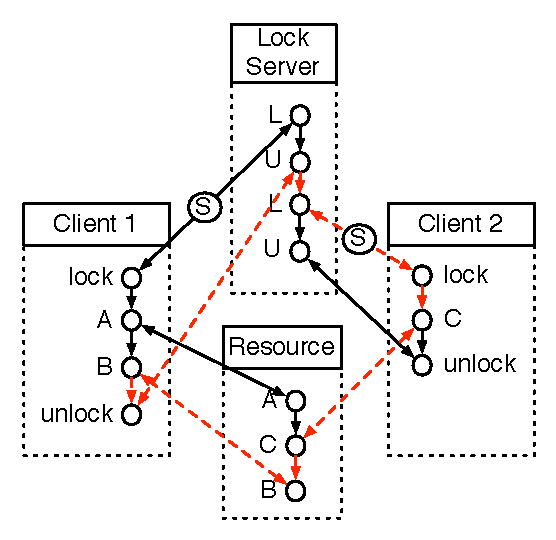
\includegraphics[width=0.5\textwidth]{Figures/OLTC}
\caption{A possible serializability violation that arises because of
asynchronous (speculative) communication with the lock server.}
\label{fig:oltc}
\end{figure}

In the absence of contention, the involvement of the lock server adds
unnecessary overhead.  By communicating with \cf{lockChan} asynchronously, we
can allow the client (the thread performing the transaction), to concurrently
proceed with obtaining other locks or executing the transaction.  Of course,
synchronous communication on the \cf{lockChan} ensures atomicity of a
transaction performed on the resource protected by the lock. However, these
guarantees are lost in the presence of asynchrony.

Consider the example presented in Figure~\ref{fig:oltc}, which shows a
serializability violation that arises because communication with the
lock server takes place asynchronously, effectively introducing speculation.
Two clients transactionally perform operations A,B and C, resp.  on a shared
resource. This resource is protected by the lock server.  Happens-before edges
are represented as directed edges. During speculative execution, clients send
lock requests speculatively, labeled \mycirc{S} on the edges, allowing them to
continue with their transactions without waiting for the lock server to
respond.

In this figure, serializability violations are captured as a cycle in the
dependence graph, represented by the dotted edges. \rxcml rejects such
executions, causing the transaction to abort, and be re-executed
non-speculatively.

\subsubsection{Results}

For our evaluation, we implemented a distributed version of this program
(\cf{vacation}) taken from the STAMP benchmark suite~\cite{STAMP}.  To adapt
the benchmark for a distributed environment, we partitioned resources into 16
\emph{shards}, each protected by a lock server.  The workload was setup for
moderate contention, and each transaction involves 10 operations. The shards
were spread across 16 EC2 M1 large instances within the same EC2 availability
zone. The clients were instantiated from all of the different regions on M1
small instances to simulate the latencies involved in a real web-application. A
benchmark run involved 10K transactions, spread equally across all of the
available clients.

\begin{figure}[t]
\centering
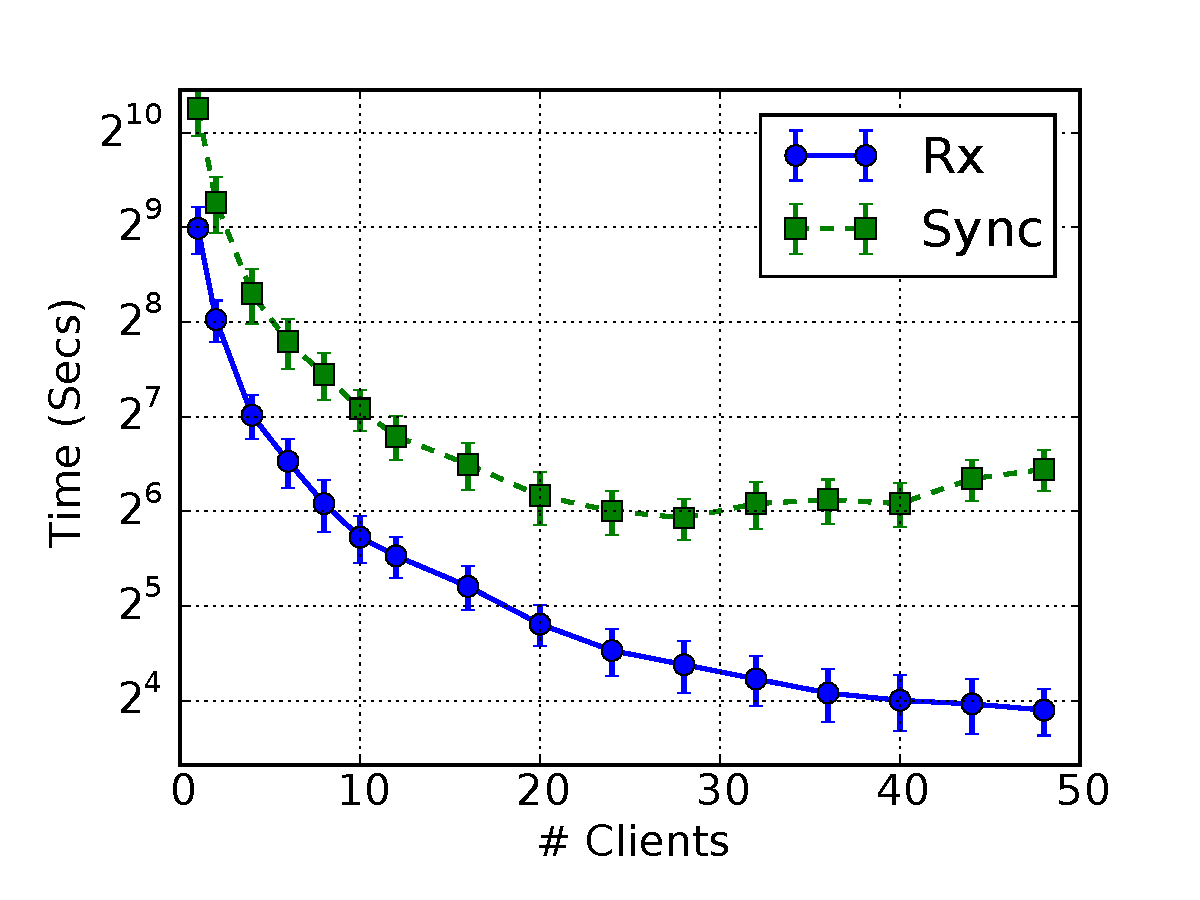
\includegraphics[width=0.5\textwidth]{Graphs/oltp_time}
\caption{Performance comparison on distributed \texttt{vacation} (OLTP)
benchmark. Lower is better.}
\label{grf:oltp}
\end{figure}

The performance results are presented in the Figure~\ref{grf:oltp}. The number
of clients concurrently issuing transaction requests was increased from 1 to
48. \rxcml is the speculative version, while Sync is the synchronous,
non-speculative variant. The 1-client Sync version took 1220 seconds to
complete. For comparison, we extended the original C version with a similar
shared distribution structure. This run was 1.3$\times$ faster than the CML
baseline. The benchmark execution under \rxcml scales much better than the
Sync version due to optimistic transactions. With 48 clients, \rxcml version
was 5.8$\times$ faster than then Sync version. Under \rxcml, the number of
transaction conflicts does increase with the number of clients. With 48
clients, 9\% of the transactions executed under \rxcml were tagged as
conflicting and re-executed non-speculatively.  This does not, however,
adversely affect scalability.

\subsection{Collaborative Editing}

Our next case study is a real-time, decentralized collaborative editing tool.
Typically, commercial offerings such as Google Docs, EtherPad, etc., utilize a
centralized server to coordinate between the authors. Not only does the server
eventually become a bottleneck, but service providers also need to store a copy
of the document, along with other personal information, which is undesirable.
We consider a fully decentralized solution, in which authors work on a local
copy of the shared document for responsiveness, with remote updates merged
incrementally. Although replicas are allowed to diverge, they are expected to
converge eventually. This convergence is achieved through \emph{operational
transformation}~\cite{SuleimanGroup97}. Dealing with operational transformation
in the absence of a centralized server is tricky~\cite{Nichols95}, and
commercial collaborative editing services like Google Wave impose additional
restrictions with respect to the frequency of remote updates~\cite{Wave} in
order to build a tractable implementation.

We simplify the design by performing \emph{causal atomic broadcast} when
sending updates to the replicas. Causal atomic broadcast ensures that the
updates are applied on all replicas in the same global order, providing a
semblance of a single centralized server.  Implemented na\"{i}vely, i.e.,
performing the broadcast synchronously, however, is an expensive operation,
requiring coordination among all replicas for every broadcast operation
compromising responsiveness. Our relaxed execution model overcomes this
inefficiency.

\begin{figure}[t]
\begin{lstlisting}
(* lc: client chan, sc: server chan, tc: timeOut chan *)
fun serverDaemon id rIn lOut =
let
	(* Updates from other server daemons *)
	val remoteRecv = wrap (brecvEvt sc, fn rOps' =>
				serverDaemon id (rIn @ rIn') lOut)
	(* Updates to other server daemons *)
	val remoteSend =
	  if lOut = [] then neverEvt ()
		else
			let val (lOut',_) = xform (lOut, rIn)
			in wrap (bsendEvt (sc, lOut', id),
  					   fn () => serverDaemon id rIn [])
			end
  (* interaction with the client *)
  val localComm =
		wrap (recvEvt tc, fn () =>
			let
				val lOps = sync
				  	(choose (recvEvt lc, alwaysEvt []))
				val (_, rIn') = xform (lOps, rIn)
				val _ = updateDocument(rIn')
			in serverDaemon id [] (lOut @ lOps)
			end)
in
  sync (choose (localComm,remoteRecv,remoteSend))
end

fun timeoutManager to =
  sync (wrap (timeoutEvent to,
	  fn () => send (tc,()); timerThread to))
\end{lstlisting}
\caption{Server Daemon for Collaborative Editing.}
\label{code:serverDaemon}
\end{figure}

The key advantage of our system is that the causal atomic broadcast is
performed speculatively, allowing client threads to remain responsive. Each
client participating in the collaborative editing session runs a server daemon,
whose implementation is given in Figure~\ref{code:serverDaemon}. The server
daemon fetches updates from the user-interface thread (client) over the channel
\cf{lc}, and coordinates with other server daemons at other remote locations
over the channel \cf{rc}.  \cf{rIn} represents the list of incoming remote
operations that have not yet been merged with the local document replica.
\cf{lOut} represents the list of local operations yet to be broadcast.

At every iteration of the server daemon loop, there is a choice (line 26) between
performing (a) a local receive (\cf{localComm}), (b) a remote send
(\cf{remoteSend}), or (c) a remote receive (\cf{remoteRecv}) (line 29). We
have extended the implementation of broadcast primitives presented in
Figure~\ref{code:bchan} with events that encapsulate broadcast send and
receive. Remote sends are only enabled if \cf{lOut} is not empty. Otherwise,
it is a \cf{neverEvt()} which will never be picked in a choice. If
\cf{lOut} is not empty, then the outstanding messages are transformed
against the remote messages and sent to all other daemons using causal atomic
broadcast (lines 11-13).

By receiving broadcasted messages on the same thread as the one that performs
the broadcast, we ensure a total order on message reception at every client.
Causal atomic broadcast ensures that all daemons receive the update in the same
order, ensuring convergence of all remote states. On receiving a remote update,
the server daemon simply appends the update to the list of pending updates yet
to be applied to the local replica (lines 5-6).

The user-interface thread sends the updates to the server daemon on the \cf{lc}
channel, making them available to other replicas. This communication is also
made asynchronous through speculation, so that the UI stays responsive to the
author. The daemon uses a \cf{timeoutManager} (lines 29-31) to periodically
fetch updates from the user interface thread. The daemon then receives local
updates \cf{lOps}, if any, from the channel \cf{lc} (lines 19-20).

Causal atomic broadcast for inter-daemon communication ensures that operations
in \cf{rIn} at every daemon appear in the same order. In other words, every
daemon is in the same abstract state. Hence, we can simply transform the
unapplied remote operations \cf{rIn} with respect to local operations
\cf{lOps}, to yield an \cf{rIn'} (line 21) that considers the remote updates in
the context of local ones.  The daemon then updates the document with the
remote operations, by applying further transformation to account for additional
local updates that might have occurred between the time the user-interface sent
a message to it and now (line 22). This operation might perform a
well-formedness check to check for consistency as updating the document is an
effectful operation. This commit prevents speculation from leaking to the user.

\subsubsection{Results}

We use a collaborative editing benchmark generator described
in~\cite{MartinAU12} to generate a random trace of operations, based on
parameters such as trace length, percentage of insertions, deletions, number of
replicas, local operation delay, etc. Our benchmarking trace contains 30K
operations, 85\%(15\%) of which are insertions(deletions), and 20\% of which
are concurrent operations. We insert a 25 ms delay between two consecutive
local operations to simulate user-interaction. Updates from each replica is
causal atomically broadcasted every 250 ms. Each replica is represented by a
\rxcml instance placed in widely distributed Amazon EC2 availability zones
chosen to capture the geo-distributed nature of collaborative editing. The
average inter-instance latency was 173 ms, with a standard deviation of 71.5.
Results are reported as the average of five runs.

\begin{figure}[t]
\centering
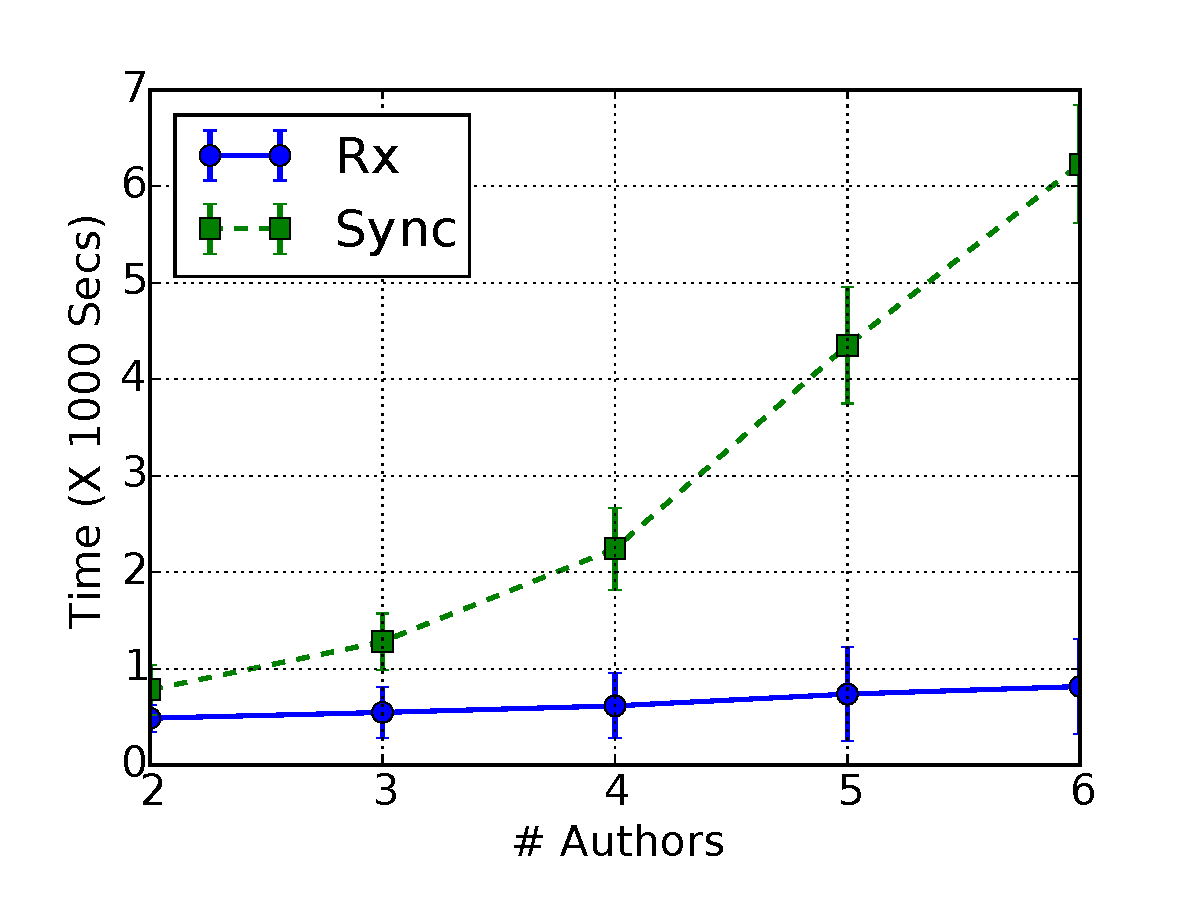
\includegraphics[width=0.6\textwidth]{Graphs/collab}
\caption{Performance comparison on collaborative editing benchmark. Lower is
better.}
\label{grf:collab}
\end{figure}

We consider the time taken by a collaborative editing session to be the time
between the first operation generation and the completion of the last broadcast
operation, at which point the documents at every replica would have converged.
Figure~\ref{grf:collab} shows results with respect to total running time. Sync
represents an ordinary CML execution, while \rxcml represents our new
implementation. With 2-authors, \rxcml version took 485 seconds to complete,
and was 37\% faster than the synchronous version. As we increase the number of
concurrent authors, the number of communication actions per broadcast operation
increases.  Hence, we expect the benchmark run to take longer to complete. The
non-speculative version scales poorly due to the increasing number of
synchronizations involved in the broadcast operations. Indeed, Sync is
7.6$\times$ slower than \rxcml when there are six concurrent authors. Not
surprisingly, \rxcml also takes longer to complete a run as we increase the
number of concurrent authors. This is because of increasing communication
actions per broadcast as well as increase in mis-speculations. However, with
six authors, it only takes 1.67$\times$ longer to complete the session when
compared to having just two authors, and illustrates the utility of speculative
communication.

\section{Related Work}

Causal-ordering of messages is considered an important building
block~\cite{Birman87} for distributed applications. Similar to our formulation,
Charron-Bost \emph{et al.}~\cite{Charron-Bost96} develop an axiomatic
formulation for causal-ordered communication primitives, although their focus
is on characterizing communication behavior and verifying communication
protocols, rather than latency hiding. Speculative execution has been shown to
be beneficial in other circumstances under high latency environments such as
distributed file systems~\cite{Nightingale05}, asynchronous virtual machine
replication~\cite{Cully08}, state machine replication~\cite{Wester09}, deadlock
detection~\cite{Li05} etc., although we are unaware of other attempts to use it
for transparently converting synchronous operations to asynchronous ones.

Besides Erlang~\cite{erlang}, there are also several distributed
implementations of functional languages that have been
proposed~\cite{DCaml,Acute}.  More recently, Cloud Haskell~\cite{CloudHaskell}
has been proposed for developing distributed Haskell programs. While all these
systems deal with issues such as type-safe serialization and fault tolerance
central to any distributed language, \rxcml's focus is on enforcing equivalence
between synchronous and asynchronous evaluation. The formalization used to
establish this equivalence is inspired by work in language and hardware memory
models~\cite{Sewell2010,Demange2013,Boehm08}.  These efforts, however, are
primarily concerned with visibility of shared-memory updates, rather than
correctness of relaxed message-passing behavior. Thus, while language memory
models~\cite{Boehm08,Demange2013} are useful in reasoning about compiler
optimizations, our relaxed communication model reasons about safe asynchronous
manifestations of synchronous protocols.

Transactional events(TE)~\cite{Donnelly06,Effinger-Dean08} combine first-class
synchronous events with an all-or-nothing semantics.  They are strictly more
expressive than CML, although such expressivity comes at the price of an
expensive runtime search procedure to find a satisfiable schedule.
Communicating memory transactions (CMT)~\cite{Lesani11} also uses speculation
to allow asynchronous message-passing communication between shared-memory
transactions, although CMT does not enforce any equivalence with a synchronous
execution. Instead, mis-speculations only arise because of a serializability
violation on memory.

\section{Concluding Remarks}

CML provides a simple, expressive, and composable set of synchronous event
combinators that facilitate concurrent programming, albeit at the price of
performance, especially in high-latency environments. This paper shows how to
regain this performance by transparently implementing synchronous operations
asynchronously, effectively treating them as speculative actions.  We formalize
the conditions under which such a transformation is sound, and describe a
distributed implementation of CML called \rxcml that incorporates these ideas.
Our reported case studies illustrate the benefits of our approach, and provide
evidence that \rxcml is a basis upon which we can build clean, robust, and
efficient distributed CML programs.
